\chapter{Literature Review}


% ------------------------------------------------------------ %


\section{Research Methodology}

The methodology aligns with the PRISMA2020 Statement, detailed in \citet{prismastatement}. In the initial ``identification'' phase, a precise research question was formulated, and search terms, alongside keywords, were curated. These were systematically employed to query the databases, saving the metadata of any retrieved matches. In the subsequent``screening'' phase, documents underwent rigorous evaluation based on their titles and abstracts to ascertain relevance. Following this, the remaining pool underwent a thorough content evaluation to determine eligibility, with any material deviating from the research focus being excluded.

The subsequent sections delineate these specific steps.

\subsection*{Identification}

The following research question was defined:

\bigskip
\textit{``In a LiDAR-based SLAM system, how can an algorithm be developed to allow the detection of both specular and transparent surfaces in real-time while being material-and-angle independent?''}
\bigskip


From this research question, four main keywords that sufficiently explain the topic were extracted: lidar, specular, detection, and slam. Furthermore, synonyms and related terms were associated to these keywords to form keyword groups as follows:

\begin{itemize}
    \item sensor:
    \begin{itemize}
        \item lidar;
        \item light detection and ranging;
        \item laser sensor.
    \end{itemize}
    \item surface:
    \begin{itemize}
        \item specular;
        \item mirror like;
        \item reflective;
        \item transparent.
    \end{itemize}
    \item goal:
    \begin{itemize}
        \item detection;
        \item identification;
        \item recognition;
        \item localization.
    \end{itemize}
    \item slam:
    \begin{itemize}
        \item slam;
        \item simultaneous localization and mapping.
    \end{itemize}
\end{itemize}

A Python script was used to automate the process of generating search strings, searching through the Scopus database, and downloading and filtering the data into an Excel sheet. It is briefly discussed in \autoref{chap:Prisma Automator}.

For instance, the subsequent three search strings are among the 144 generated:
\begin{itemize}
    \item ``lidar'' AND ``reflective'' AND ``detection";
    \item ``light detection and ranging'' AND ``specular'' AND ``localization'' AND ``slam";
    \item ``laser sensor'' AND ``transparent'' AND ``recognition'' AND ``slam".
\end{itemize}

The Scopus search yielded a total of $606$ documents. Within this pool, $288$ duplicates and $19$ conference reviews were identified, amounting to a sum of $307$ automatically excluded documents.

\subsection*{Screening}

Various factors were taken into account for the exclusion of documents:
\begin{enumerate}
    \item problem and goal were too different (e.g., building new hardware, analysis of leaf reflectance);
    \item not sufficiently related to this work (e.g., focused on hyperspectral \gls{lidar});
    \item duplicates that were not automatically detected and excluded.
\end{enumerate}

\textcolor{red}{The following needs to be fixed!}
Finally, only 12 documents remained in the pool. Out of those, 5 were not retrievable (required a subscription) and 3 were not eligible due to not being sufficiently related to this work. Only 4 papers remained. A summary of the whole process can be found in \autoref{fig:prisma}.

Other 13 documents were also manually included through snowball search or as suggestions from field experts. The following section discusses those that were of most interest to this work.


\begin{figure}[htb]
    \begin{center}
        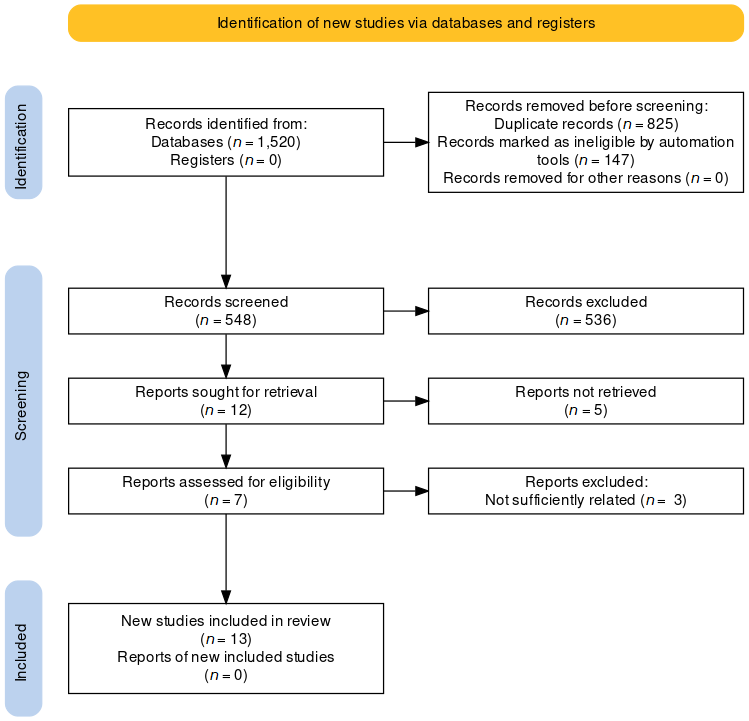
\includegraphics[width=1\textwidth]{img/prisma.png}
    \end{center}
    \caption{\label{fig:prisma}PRISMA Flow Diagram. Source: author.}
\end{figure}


% ------------------------------------------------------------ %


\section{State of the art}
\textcolor{red}{[WIP]``Glass like surface detection has gained traction this past decade (?) ... techniques like dual return, sensor fusion, intensity, etc are popular and considered state of the art ... X (2022) used LiDAR sensors and their laser intensity to build a probabilistic profile for identifying glass whenever peaks show up ... Y (2023) utilizes LiDARs with dual-return for detecting anomalies in the intensity profile ..."}




% ------------------------------------------------------------ %


\section{Research deficit}
\textcolor{red}{[WIP] All of the discussed techniques are limited by one or more of the following constraints: angle has to be close to normal; the model works only under specific lighting conditions; the algorithm can only identify specific materials of glass; either the reflection or transparency problem is solved, but not both; etc. ... furthermore, these tecniques are often not real-time performant ... open-source implementations are rare and lacking on today's most popular robot programming framework, ROS ...}